\documentclass[10pt, article]{llncs}

\newcommand{\highlight}[1]{\colorbox{yellow}{#1}}


% Some very useful LaTeX packages include:

% *** MISC UTILITY PACKAGES ***
%
\usepackage{ifpdf}


% *** MATH PACKAGES ***
%
\usepackage[cmex10]{amsmath}
\usepackage{amssymb}

% *** SPECIALIZED LIST PACKAGES ***
%
\usepackage{algorithmic}


% *** ALIGNMENT PACKAGES ***
%
\usepackage{array}

% *** SUBFIGURE PACKAGES ***
%
\usepackage[tight,footnotesize]{subfigure}
\usepackage{subfig}

% *** FLOAT PACKAGES ***
%
\usepackage{fixltx2e}
\usepackage{stfloats}

% *** GRAPHICS PACKAGES ***
%
\usepackage{graphicx}

% *** BIBLIOGRAPHY PACKAGES ***
%
\usepackage{natbib}

% *** LANGUAGE PACKAGES ***
%
\usepackage[utf8]{inputenc} 
\usepackage[T1]{fontenc}      
\usepackage[french]{babel}

% *** LAYOUT PACKAGES ***
%
\usepackage[top=4cm, bottom=4cm, left=4cm, right=4cm]{geometry}

% *** PAGE NUMBERING PACKAGES ***
%
\usepackage{fancyhdr}
\usepackage{lastpage}

% *** HEADER AND FOOTER ***
%
\pagestyle{fancy}
\fancyhf{}
\lhead{\rightmark}
\cfoot{Page \thepage \hspace{1pt} sur \pageref{LastPage}}
\pagenumbering{arabic}


\begin{document}
%
% paper title
\title{Les Citizen Sciences dans\\l'accomplissement des SDG's : \\un exemple environnemental}



% author names and affiliations
% 
\author{Djavan Sergent \\
Superviseur : François Grey\\
Master en Sciences Informatiques \\
djavan.sergent@etu.unige.ch}

\institute{Université de Genève}



% make the title area
\maketitle

\begin{abstract}
	<ABSTRACT>
\end{abstract}


\textbf{Mots clés} Citizen Science ; Monitoring ; Water Quality ; Sustainable Development

\pagebreak

\section{Introduction}
	En 2000, les Nations-Unies lancent le programme des Millenim Developpment Goals (MDGs) qui s'étend jusqu'en 2015 \cite{united_nations_millennium_2009}. Il s'agit d'un ensemble d'objectifs internationaux parmi lesquels on peut notamment citer l'éradication de l'extrême pauvreté et de la faim, combattre la mortalité infantile ou encore apporter une éducation à toutes et tous. Les 191 états membres des Nations-Unies ainsi que 22 organisations internationnales se sont engagées à participer activement à la réalisation de ces objectifs \cite{wikipedia_millennium_2017}.
	
	Fin 2015, beaucoup d'efforts ont été investis, mais les progrès sont encore très inégaux. Les différents pays membres des Nations-Unies ainsi que des organisations civiles se sont donc intéressées à l'agenda post-2015, c'est à dire aux objectifs futurs. Les Sustainable Developpment Goals (SDGs) ont étés acceptés comme relève des MDGs \cite{wikipedia_sustainable_2017}. Ceux-ci comportent 17 buts, chacuns subdivisé en objectifs. Les SDGs totalisent 169 objectifs qui possédent tous leurs propres indicateurs.
	\begin{figure}
		\begin{center}
			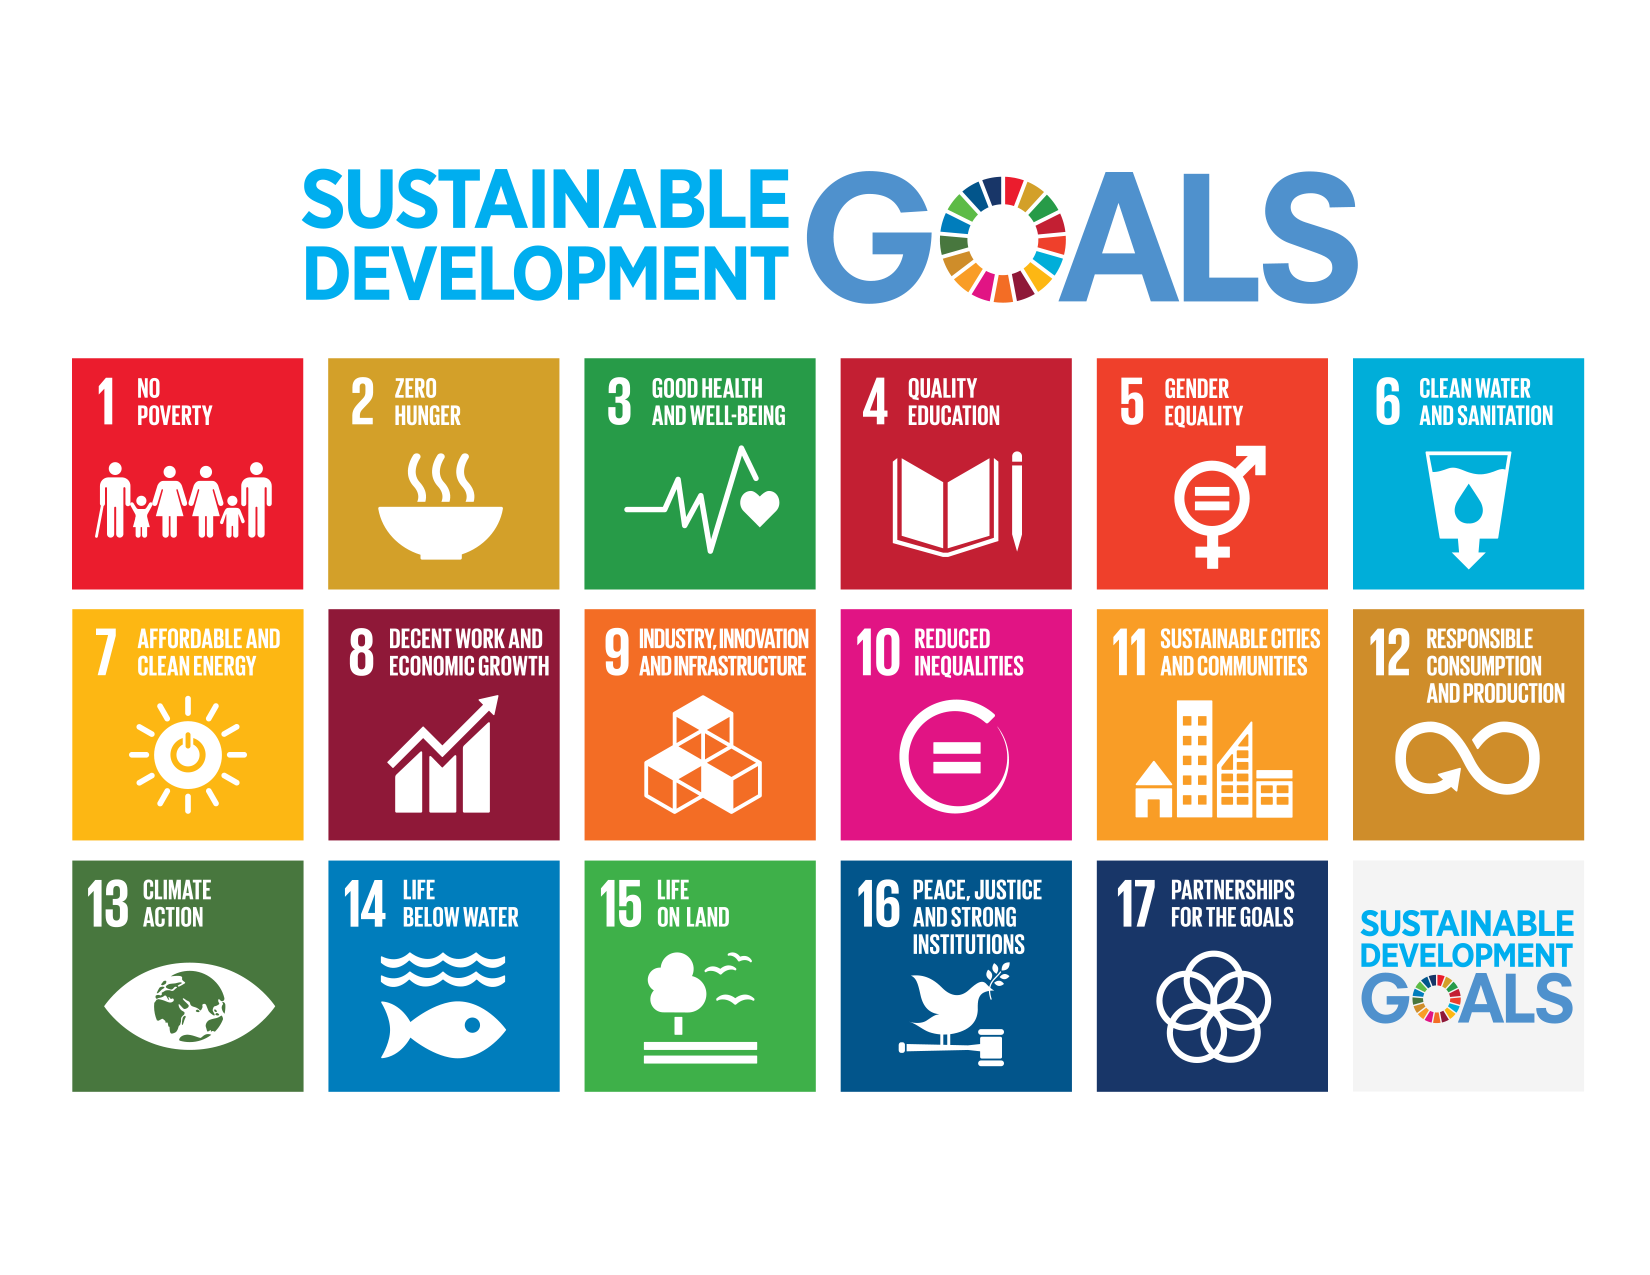
\includegraphics[width=300pt]{img/sdgs.png}
		\end{center}
		\caption{Icônes des SDGs (source : Sustainable Development Knowledge Platform)}
	\end{figure}
	Nous analysons dans cet article le rôle du numérique dans la réalisation des certains SDGs, particulièrement du point de vue de la participation citoyenne. Une attention spéciale est portée sur la qualité de l'eau et de l'air, sur les différents indicateurs qui permettent de l'évaluer et sur les méthodes de surveillance utilisé tant au niveau global que local au moyen de prélèvements.

\section{Sustainable Developpment Goals}
		Les SDG's sont en ensemble de buts à atteindre pour répondre à plusieurs problématiques mondiales. Ces buts s'intéressent autant à l'égalité homme-femme qu'à l'éradication de la pauvreté ou encore la restauration des écosystèmes. Ces objectifs sont pensés pour être revus régulièrement afin d'analyser les progrès effectués et les éventuelles modification de la feuille de route. En moyenne, chaque objectif est revu tous les deux ans. \\
		Les points prioritaires des SDG's ont été de développer rapidement les aspects ci-dessous \cite{lu_policy:_2015} :
		\begin{itemize}
			\item Définir les métriques : Il est important que les communauté scientifiques, économiques et sociales puisse surveiller et traquer les progrès réalisés au sein de chaque SDG au moyen de métriques standardisés
			\item Etablir des mécanismes de surveillance : En mettant en place le système permettant de mesurer les indicateurs qui définissent les métriques. Une collaboration active entre les gouvernements et entre les scientifiques est indispensable à la mise en place de programmes de surveillance. 
			\item Evaluer les progrès : Il faut évaluer les progrès effectués et vérifier que les objectifs répondent toujours au problème. Cela permet également de surveiller les indicateurs les plus pertinents en fonction du mode de gouvernance (rapport qualité/prix, égalité sociale, etc.).
			\item Améliorer l'infrastructure : Afin de pouvoir couvrir une zone toujours plus large et avoir une vision plus globale, il faut apporter une attention particulière aux investissements dans les différentes infrastructures. Pour cela, des partenariats sont nécessaires (Futur Earth, World Meteorological Organization, etc.). Le recours aux smartphones est également un excellent point de départ pour multiplier les possibilités et opportunités de surveillance environnementale.
			\item Données standardisées et vérifiées : Il est crucial que les données soient standardisées pour être comparables au niveau international. Toutes les données doivent être vérifiées et rendues publiques le plus rapidement possible.
		\end{itemize}
		\subsection{Objectifs}
			Nous nous intéressons, dans le cadre de cet article, aux buts décrits ci-dessous. Il est cependant important de noter que les objectifs sont intrinséquement liés entre eux et s'influencent mutuellement. Par exemple, en formant des citoyens à l'utilisation de matériel de mesure de qualité de l'eau, on va agir non seulement sur la capacité à, entre autre, détecter la pollution mais également sur l'éducation qui est au coeur d'un autre objectif.
			\begin{description}
				\item[ 3 - Good Health and Well-Being :] La santé et la pollution de l'air sont au centre de ce but.
				\item[ 6 - Clean water and sanitation :] Un accès universel à l'eau et aux installations sanitaires est essentiel pour la santé humaine, la prospérité économique et la préservation de l'environnement.
				\item[14 - Life below water :] L'acidification des océans, la surpêche ou encore la pollution marine ont un impact important sur la protection des océans. Leur dégradation provoque des effets sur certaines espèces marines mais également sur la biodiversité et le fonctionnement des écosystèmes.
			\end{description}				
		
		\subsection{Progrès, revue et indicateurs}
			Le High-Level Political Forum (HLPF), créé en 2012 à la suite de Rio20+, est chargé de promouvoir les objectifs, d'assurer un suivi et d'émettre des recommandations pour la réalisation des SDGs. Ce forum se réunit annuellement. \\
			Les dix-sept buts possèdent leurs propres indicateurs globaux et standardisés. Ces indicateurs servent à évaluer les progrès effectués au niveau international, national, régional et local. \\
			Le HLPF revoit une partie des objectifs lors des réunions annuelles, les autres sont abordés à une session ultérieure. La participation et la collaboration est revue chaque année pour favoriser le développement des SDGs.\cite{united_nations_high-level_nodate}

\section{Surveillance environnementale}
	\subsection{Eau}
			L'eau est l'une des ressources naturelles les plus importante sur terre. Elle joue un rôle essentiel dans de multiples secteurs économiques, sanitaires et environnementaux.\\
			L'accès à l'eau potable, à des installations sanitaires et un plan de gestion des ressources est un enjeu majeur des SDGs. Réparties de façon inégale sur terre \cite{lefevre_repartition_nodate}
			, l'eau est essentielle pour le développement économique, l'agriculture, la protection de l'environnement ou encore la santé. Dans de nombreux pays tels que les États-Unis, la plus grande partie de cette eau est dédiée à l'agriculture \cite{world_business_council_for_sustainable_development_global_nodate}.
			Dans ce contexte, il est important de mettre en oeuvre des systèmes de gestion des ressources hydriques et de permettre un accès universel à des sources d'eau propre. Ce but a un impact sur d'autres tels que la santé ou la lutte contre la faim.
			\begin{figure}
				\begin{center}
					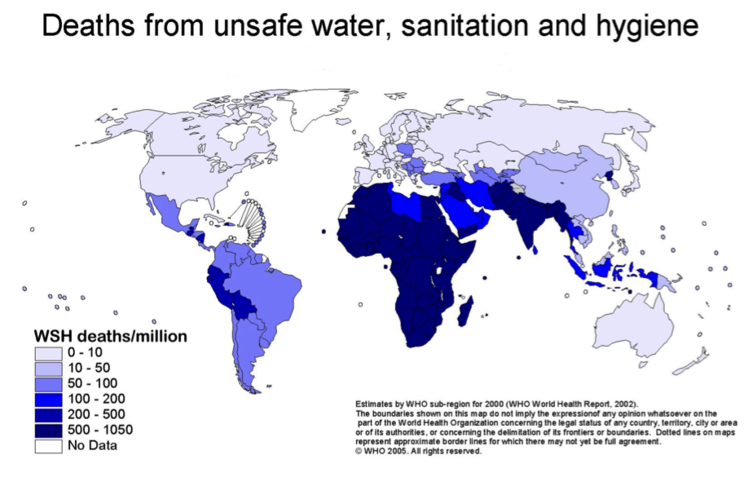
\includegraphics[width=250pt]{img/water_deaths_2002.png}
				\end{center}
				\caption{Morts à cause de la qualité de l'eau par pays en 2002 (source : World Health Organisation)}
			\end{figure}
			Selon les rapports du secrétaire-général du conseil économique et social des Nations-Unies \cite{united_nations_economic_and_social_council_progress_2017}\cite{united_nations_economic_and_social_council_progress_2017-1}, un tiers de la population mondiale n'a, en 2015, pas accès à des installations sanitaires. Selon les même rapports, parmi eux, 946 millions n'ont accès à aucune infrastructure. La mauvaise gestion des déchêts humains représente un risque concret pour la santé et pour l'environnement \cite{ashbolt_microbial_2004}.\\
			Concernant l'accès à l'eau potable, la situation évolue positivement. On constate qu'en 2000, 82 pourcent de la population dispose d'une source d'eau aménagée contre 91\% en 2015. Cependant, on estime également qu'environ 25\% de la population mondiale est exposée à de l'eau contaminée par des matières fécales \cite{united_nations_goal_nodate-4}. \\
			Selon le rapport \cite{rana_water_2017}, il n'existe pas de plan complet qui permette la mise en place d'un système de gestion renouvelable des ressources en eau et le manque de données précises rend impossible l'évaluation des performances pour les approches actuellement implémentées. \\
			Toujours d'après ce même rapport, les innondations sont à l'origine de nombreuses maladies et dommages causés à des infrastructures. Les innondations peuvent causer des épidémies, comme le démontre le cas de Itaparica Dam au Brésil lors duquel, en 1988, plus de 2000 cas de gastroantérite sont déclarés sur une période de 42 jours. 88 d'entre eux s'avéreront mortels. Les innondations favorisent également la reproduction des moustiques et ainsi la propagation de maladies telles que la Rift Valley Fever (RFV) \cite{hanafi_rift_2010}.\\
			Un aspect également très important de la gestion de l'eau concerne les "Dead Zones" qui s'étendent de façon exponnentielle depuis 1960 \cite{diaz_spreading_2008}. Les "Dead Zones" sont de larges étendues d'eau qui n'ont plus assez d'oxygène pour assurer la vie marine. En 2008, 400 de ces zones affectant plus de 245'000km$^{2}$, majoritairement situées dans les océans, sont répertoriées. La cause principale du développement des "Dead Zones" est la libération dans l'eau de nutriments qui accélèrent la croissance de certaines algues, réduisant la quantité d'oxygène disponible sous la surface. Bien que ces zones soient souvent d'origine naturelle, leur croissance est particulièrement accélérée par la proximité de sites industriels et agricoles qui rejettent leurs nutriments dans l'eau.
			\begin{figure}
				\begin{center}
					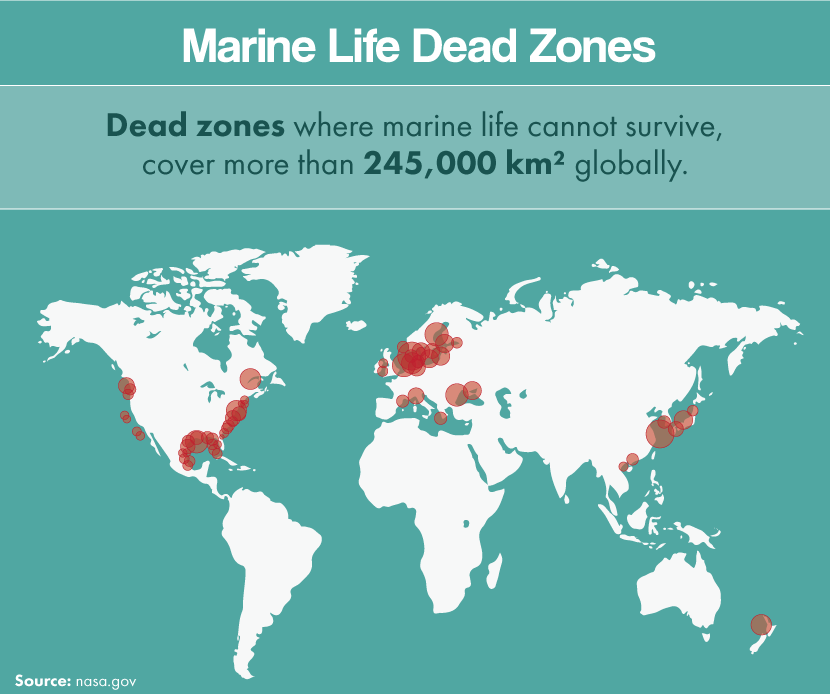
\includegraphics[width=200pt]{img/marine-life-dead-zones.png}
				\end{center}
				\caption{Répartition des zones mortes (source : nasa.gov)}
			\end{figure}
			Autre constat : certains pays dépassent en consommation la quantité d'eau renouvelable à disposition et exercent donc une pression sur le cycle de l'eau. \\
			La multitude de problématiques présentées ci-dessus explique pourquoi l'eau est au coeur des SDGs. Depuis de très nombreuses années, une attention particulière est portée à la qualité de l'eau et aux dangers liés à une contamination de celle-ci \cite{ashbolt_microbial_2004}. Le manque d'infrastructures sanitaires dans les régions en développement les rends vulnérables aux morts par contamination de l'eau. Neuf morts sur dix touchent les enfants, et tous les décès surviennent dans ces régions. \\
			Aujourd'hui, de nombreux outils permettent de suivre avec précision les indicateurs classiques de qualité de l'eau tels que le taux d'oxygène, l'acidité, la température, la conductivité etc. Ceci est très important pour la réalisation du but 6.3 : <<By 2030, improve water quality by reducing pollution, eliminating dumping and minimizing release of hazardous chemicals and materials, halving the proportion of untreated wastewater and substantially increasing recycling and safe reuse globally>> \cite{united_nations_goal_nodate-4}. \\
		
		\subsection{Air}
			La qualité de l'air est aujourd'hui responsable de nombreuses maladies, cancers et décès. Une étude chinoise récente met en avant l'augmentation de la fréquence de visite des hopitaux pour des problèmes respiratoires lors de l'augmentation du nombre de particules fines dans l'air \cite{liu_effects_2016}. La réduction du nombre de morts attribuables à la qualité de l'air est un des indicateurs de l'objectif 3 (Good-Health and Well-Being) \cite{united_nations_goal_nodate-5}. En opposition à la qualité de l'eau, celle de l'air s'est dégradée lors de la dernière décennie. En 2012, la pollution de l'air est responsable d'environ 5.5 milions de morts à travers le monde et environ la moitié de la population mondiale est exposée à un air dont la concentration en particules fines est supérieure à 10 microgrammes/m$^{3}$ \cite{yale_university_epi_2016}. Certains chercheurs affirment aussi qu'on peut constater un lien entre le nombre de tumeurs malignes du cerveau dans une région géographique et son taux de particules fines \cite{andersen_long-term_nodate}. \\
			\begin{figure}
				\begin{center}
					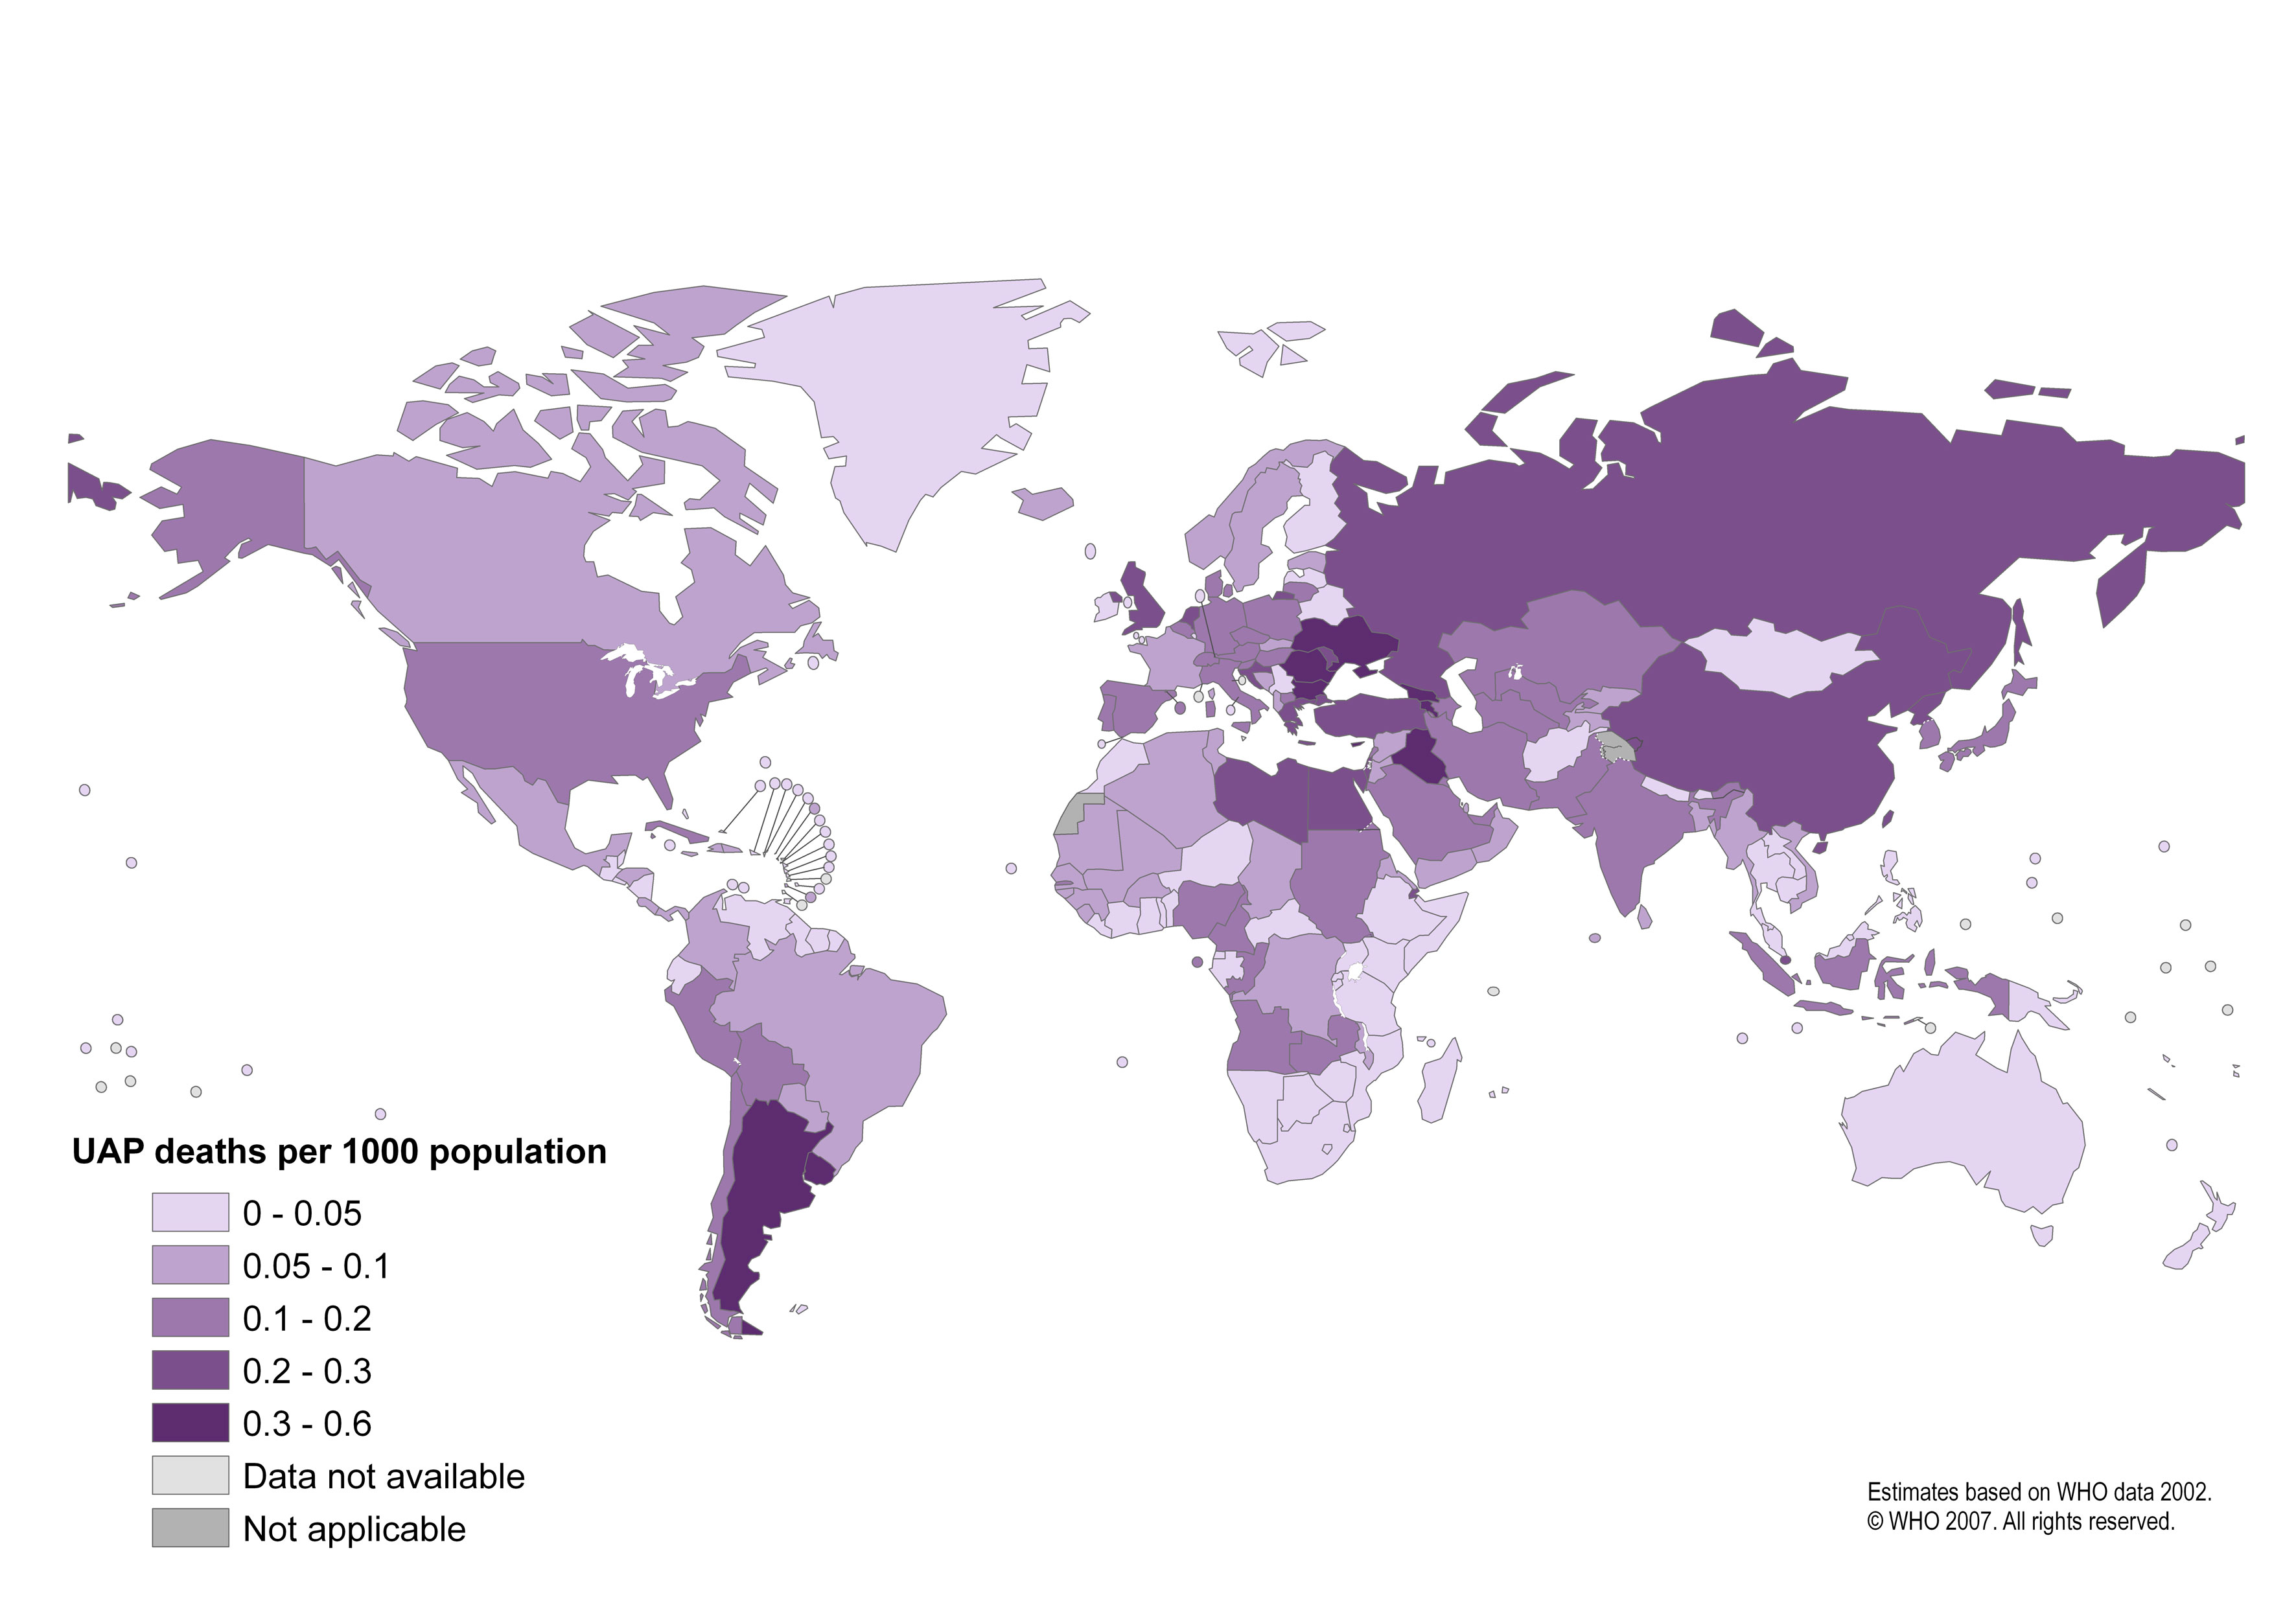
\includegraphics[width=200pt]{img/pollution-deaths-by-1000-population.jpg}
				\end{center}
				\caption{Morts à cause de la qualité de l'air par pays en 2012 (source : World Health Organisation)}
			\end{figure}
			La pollution de l'air impacte également le changement climatique en modifiant la composition de l'atmosphère et des océans. L'augmentation de la quantité de CO$_{2}$ dans l'air influe sur l'acidité des océans et impacte donc les espèces marines sensibles à ces changements. La modification de la composition chimique des océans affecte directement la reproduction de certaines espèces marines et la capacité des espèces de cnidères, tels que les coraux, à créer leur exosquelette \cite{hoegh-guldberg_coral_2007}.  \\		
		
		\subsection{Bio-indicateurs}
			Depuis les années 1970, les auteurs de diverses études \cite{archaimbault_indice_2010} analysent les relations entre la faune et la qualité environnementale de leurs habitats. On considère en effet que les relevés sont capables de fournir des indicateurs sur l'état et la qualité de l'écosystème aquatique étudié. Dès lors, on a mis au point de nombreux outils basés sur les macro-invertébrés benthiques a des fins de diagnostiques concernant la qualité des écosystèmes aquatiques.\\
			En Europe, les macro-invertébrés benthiques sont les éléments les plus utilisés pour comprendre, analyser et révéler les pressions anthropiques exercées car ils présentent les caractéristiques suivantes :
			\begin{itemize}
				\item Ils sontrelativement sédentaires et certains sont extrêment sensibles ou résistants aux perturbations et pollutions importantes.
				\item Ils sont très hétérogènes, la plupart du temps abondants et disposent d'une grande variété de formes et d'espèces.
				\item Pour une variation environnementale donnée, il est très probable de trouver quelques organismes qui réagissent fortement et, souvent, de façon extrêmement rapide.
				\item La différence de caractéristiques entre les différents organismes va modifier leur réponse en fonction de la nature et de l'intensité du stress.
				\item Leur durée de vie qui varie de quelques mois à quelques années est suffisante pour enregistrer et surveiller la qualité environnementale.
				\item On peut trouver des macro-invertébrés benthiques de façon abondante dans tous les types d'habitats.
				\item Ils sont relativement aisés à collecter et présentent l'avantage, par rapport aux micro-organismes et au plancton, d'être bien plus facile à identifier.
			\end{itemize}
			L'IBGN est un des outils diagnistiques de la qualité des écosystèmes aquatiques qui utilise les macro-invertébrés benthiques pour leurs nombreuses caractéristiques. \\
			Le protocole de l'IBGN impose un échantillonage en 8 prélèvements réalisés sur des substrats différents, dans un ordre défini par la norme et en tenant compte de la vitesse du courant. On utilise un filet de type Surber d'une surface d' 1/20$^e$ de m$^2$ et donc les mailles mesurent 500$\mu$m. On calcule l'indice en estimant différents paramètres en utilisant une liste finie de 152 taxons. Parmi ces 152 taxons, 38 seront considérés comme indicateurs et permettent la définition de 9 groupes faunistiques correspondant à leur pollusensibilité. Le calcul se fait alors en 3 étapes :
			\begin{enumerate}
				\item On détermine la "classe de variété taxonomique" (A) qui est égale au nombre de taxons récoltés sur les 152 potentiellement présents. Un taxon est considéré présent même s'il est représenté par un seul individu.
				\item On détermine le "groupe faunistique indicateur" (B) en ne prenant en compte que les taxons indicateurs. Il doit y avoir au moins 3 individus (ou 10 pour certains taxons) par échantillon.
				\item L'indice est obtenu par la formule suivante : $A + (B - 1)$ avec $IBGN \le 20$
			\end{enumerate}
			\begin{figure}
				\begin{center}
					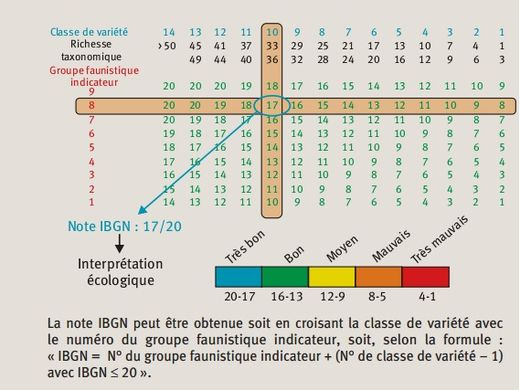
\includegraphics[width=300pt]{img/ibgn.jpg}
				\end{center}
				\caption{Calcul de l'IBGN (source : \cite{ibgn})}
			\end{figure}
			L'intérêt de cette méthode réside dans le fait qu'elle tient compte de toutes les communautés d'invertebrés et non pas uniquement des groupes les plus sensibles. Il est relativement aisé de récolter, manipuler et exploiter les informations. De plus, il est adapté au suivi de la qualité écologique d'un point d'eau de part ses larges possibilités d'applications. Le protocole permet de suivre spatialement les variations et perturbations, d'en suivre l'évolution à travers le temps ou de considérer le point d'eau isolément.
			Cependant, cette méthode d'analyse n'est pas adaptée aux zones sources et/ou profondes et ne permet pas d'évaluer la variabilité saisonnière liée aux cycles biologiques. Il n'est pas possible non plus d'identifier la nature exacte de la perturbation observée. De plus, certaines zones comme les rivières de haute montagne dont la diversité naturelle est faible on un indice inférieur à l'indice de référence ($IBGN = 20$) en dehors de toute perturbation. Pour les cours d'eau profonds, on préfère utiliser l'indice IBGA qui modifie légèrement le protocole de prélèvement en en effectuant certains par draguage. Lorsqu'il n'est pas possible d'effectuer un draguage (fonds encombrés et/ou navigation trop importante) on utilise la méthode IQBP qui consiste à laisser un piège à benthiques 1 mois au fond de l'eau pour que ceux-ci le colonisent. Les indices IBGA et IQBP sont également basés sur une note sur 20 établie sur l'analyse de la faune benthique.
		
		\subsection{Réseaux de capteurs autonomes sans fils}
			Les réseaux de capteurs sans fils (Wireless Autonomous Sensor Network - WASN) sont des réseaux dont les capteurs sont distribués dans l'espace et le temps. La spécificité de ce type de réseau est qu'ils doivent pouvoir se montrer redondants face à une défaillance de l'un des noeuds du réseau. Le routage de l'information doit être optimisé pour favoriser la durée de vie du réseau. On considère en effet que les différents noeuds disposent d'une source d'énergie limitée avant de devoir être rechargés, supprimés ou remplacés. La transmission d'information par radio-fréquence est extrêmement coûteuse en énergie, c'est pourquoi il existe de nombreux algorithmes permettant d'optimiser la consommation du réseau localement mais aussi globalement. D'autres algorithmes permettent aux capteurs de se situer spacialement pour appliquer les différents protocoles de routage possibles.\\
			Ces réseaux sont très intéressants dans le cadre du monitoring environnemental puisqu'ils permettent de couvrir de large étendues. \cite{professor_course_nodate}
		
\section{Participation citoyenne}
	Les citoyens peuvent contribuer à la réalisation de ces SDGs par plusieurs moyens, qu'il s'agisse de la récupération, du traitement des données receuillies sur le terrain, de la mise à disposition de ressources ou d'outils \cite{lordkipanidze_che_nodate}. On peut citer en exemple le "World Water Monitoring Day", journée lors de laquelle des miliers de citoyens vont récupérer, dans les points d'eau proche de chez eux, des échantillonsdont la qualité est analysée. \\
	Lorsque l'étendue géographique à couvrir et/ou la durée des observations dans le temps sont des paramètres importants, il est intéressant de recourir à un nombre important de citoyens bénévoles non spécialistes plutôt qu'à un petit groupe d'expert. De plus, leur nombre et leur répartition sur le terrain permettent de limiter les risques financiers, de biais et d'évaluation non-neutre. Des protocoles standardisés sont nécessaires dans cette approche citoyenne.\\
	Il y a aujourd'hui un réel besoin d'incorporer les données récoltées par les sociétés civiles aux SDG's \cite{fluckiger_sustainable_2016}.\\
	Les citoyens ordinaires peuvent également proposer des solutions innovantes comme le démontre Jeff Bass au moyen de son réseau autonome de 13 Respberry Pi utilisés dans sa ferme Californienne afin de mesurer la quantité d'eau utilisée, détecter les fuites et recevoir des alertes lorsque l'utilisation de l'eau est anormale.\\
	Les exemples ci-dessous représentent un échantillon parmi la multitude de projets citoyens et d'études menés à travers le monde. Ils ont pour but de donner une idée des opportunités offertes par les nouvelles technologies à bas prix lorsqu'elles sont utilisées dans un contexte de sciences citoyenne.
	
	\subsection{Citizen Cyberlab}
		Citizen Cyberlab (voir \textit{citizencyberlab.org}) est une organisation créée en collaboration avec le Centre Européen de Recherche Nucléaire (CERN), l'United Nations Institute for Training And Research (unitar) et l'Université de Genève qui participe activement à la recherche de nouvelles possibilités pour que les citoyens puissent participer à la recherche. Citizen Cyberlab agit sur des projets classés en quatres catégories (computing, thinking, sensing, understanding) en fonction de leur objectif prioritaire. Tous les projets sont orientés pour respecter les normes Open Science, c'est à dire du matériel, des logiciels, des formats de données et des publications libres.\\
		L'un des projets de la catégorie computing se nomme "Computing for Clean Water". Il est mené en collaboration avec l'IBM World Community Grid et un centre multidisciplinaire de l'Université de Tsinghua et a pour ambition de modéliser et comprendre les propriétés moléculaires de nouvelles classes de filtres à eau efficaces et bon marché destinés à aider à répondre à la demande d'eau peu chère, propre et consommable. Ces filtres, développés en collaboration avec de nombreuses universités, sont constitués de nanotubes de carbones qui réduisent la friction de l'eau sous certaines conditions et permettent une amélioration de la diffusion de l'eau de près de 300\% Cette étude se base sur une simulation de plusieurs années qui requiert environ 40'000 années de calculs sur un ordinateur personnel standard. L'utilisation du public a déjà permit de réduire de façon significative le nombre d'années nécessaires et les coûts pour les scientifiques puisqu'ils ont pu bénéficier de la puissance de calcul de près de 3 millions d'ordinateurs répartis à travers le monde grâce à l'IBM World Community Grid. Si les calculs avaient été effectués de façon commerciale, ils auraient couté environ 15 millions de dollars américains. Le projet vise désormais à une meilleure compréhension du phénomène physique à l'origine de cette amélioration de la diffusion de l'eau à travers les nanotubes.\\
		Un autre projet, qui fait partie de la catégorie thinking, se nomme Open Seventeen (O17). Il s'agit d'un programme de coaching pour les projets inovateurs qui permettent d'atteindre les buts fixés par les SDG's. O17 veut encourager la participation du public et les sciences citoyennes. Un cycle de O17 se présente comme ceci : un appel aux projets permettant de répondre à un problème concret est lancé. Une sélection se fait sur l'ensemble des projets reçus et les plus prometteurs sont regroupés en équipes. Les équipes bénéficient ensuite d'un coaching particulier par des experts et coachs internationaux sur une durée de six semaines pour transformer leur idée en projet viable. A la fin de ces six semaines, les projets les plus prometteurs recoivent une aide plus avancée pour le développement et la concrétisation du projet.
		
	\subsection{Public Lab}
		Public Lab (voir \textit{publiclab.org}) est un réseau américain de sciences citoyennes. Ils développent du matériel et des logiciels qui sont ensuite utilisés dans des projets de sciences citoyennes. Ils sont à l'origine de nombreux projets tels que l'Open Water Project, Open Air, Open Land, etc. et contribuent à d'autres tel que l'InfoAmazonia en participant à l'élaboration des composants utilisés dans le capteur Mae d'Agua.\\
		Public Lab a créé de nombreux capteurs spécialisés dans l'analyse des données environnementales. Le Riffle est designé pour être étanche, open source, open hardware et compatible avec un Arduino. Il permet initialement de mesurer la température de l'eau, mais il est également modulable et on peut lui ajouter des capteurs de turbidité, de pression et de conductivité. Cette modularité et son prix relativement bas lui offre une large variété de cas d'utilisation. Le Riffle est pensé pour répondre aux critères suivants :
		\begin{figure}
			\begin{center}
				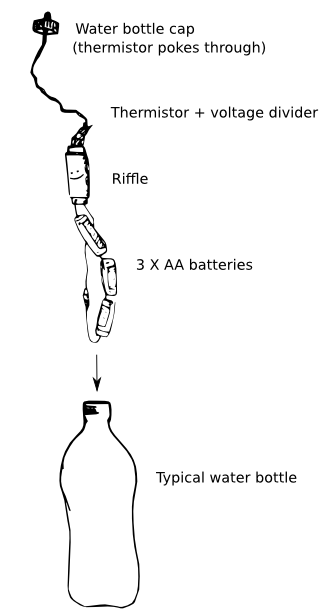
\includegraphics[width=100pt]{img/bottle_enclosure.png}
			\end{center}
			\caption{Idée générale de l'encapsulation du Riffle, de son alimentation en électricité et ddes différents capteurs (source : Public Lab)}
		\end{figure}
		\begin{itemize}
			\item Faible consommation de batterie : le capteur doit pouvoir fonctionner au moins une semaine sans être rechargé.
			\item Du matériel libre : pour permettre à la communauté de le modifier et en faciliant l'ajout de nouveaux capteurs.
			\item Des logiciels libres : qui ont pour but de faciliter le transfert et la visualisation d'informations.
			\item Matériel de stockage libre : pour que les données de sorties soient au format CSV et sur une carte SD.
			\item Du matériel accessible : il doit être facile de remplacer un composant, et si possible de le trouver localement. Le tout doit pouvoir être encapsulé dans un conteneur étanche.
			\item Créer une communauté : en engageant des citoyens autour de la création d'un tel objet.
		\end{itemize}
		Le plus grand challenge est de trouver un conteneur étanche qui permette la réalisation des relevés désirés. Plusieurs approches plus ou moins satisfaisante sont proposées, mais la plus intéressante propose d'utiliser de simples bouteilles en plastique dont on perce le bouchon pour laisser sortir les capteurs.
		Cette configuration a donné lieu à de nombreuses propositions comme l'utilisation de riz pour absorber les éventuelles fuites, ou encore l'ajout de capteurs de conductivité (qui n'étaient pas prévus dans le design initial). Il existe également des plans d'impression 3D pour imprimer un conteneur étanche sur la base d'une capsule en PVC.\\
		La carte possédant le circuit électronique a été développée pour être entièrement compatible avec l'IDE d'Arduino et d'une size qui lui permette de passer dans la plupart des goulots des bouteilles de 20mm. Le fait de devoir glisser le tout par l'embouchure demande également à ce que les broches de connexion se trouvent aux extrêmités de la carte afin que les cables passent verticalement.
		\begin{figure}
			\begin{center}
				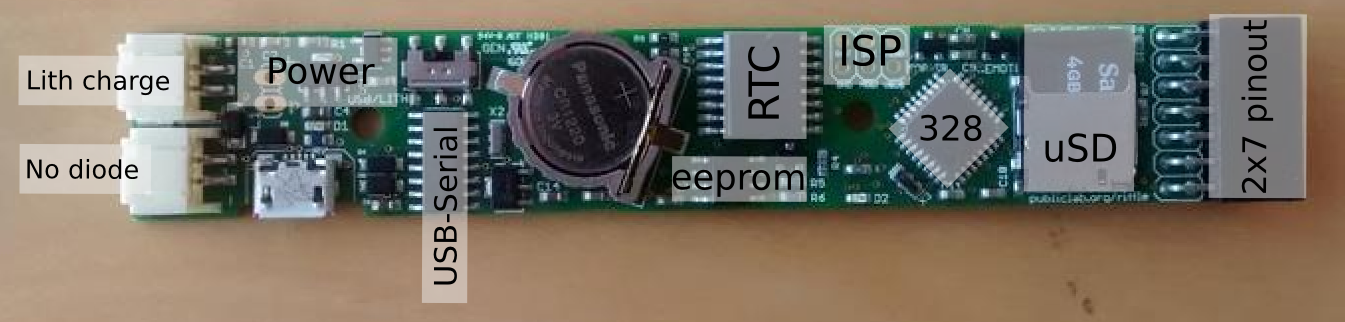
\includegraphics[width=300pt]{img/riffle_parts_2.png}
			\end{center}
			\caption{Dernière version du Riffle (source : Public Lab)}
		\end{figure}
		La configuration du Riffle est hautement modulable et permet par exemple l'ajout d'une carte GSM ou d'un émetteur/récepteur radio pour les télécommunications.  Le problème d'une carte SIM étant bien sûr les coûts mensuels liés à son utilisation. A noter que les télécommunications ont également un effet non négligeable sur la durée de vie d'un appareil. Les interfaces utilisées sont sélectionnées pour être compatibles avec la plus large variété de protocoles et de matériel électroniques externes. Les données recueillies sont ensuite fournies au format CSV ou TSV et c'est à l'utilisateur de voir comment il veut les traiter. Cette décision a été prise après discussion avec de nombreux hydrologues car il existe de nombreux workflows différents. Il est donc plus pertinent de présenter les données sous un format générique et de laisser le soin de les rendre compatible avec son propre système à l'utilisateur.\\
		Public Lab a également contribué à d'autres projets comme le Thermal Fishing Bob (capteur de température basé sur la lumière), le Coqui qui peut émettre des fréquences de son audibles et effectuer des mesures de conductivité, de température et de visibilité, ou le Kit Initiative qui vise à mettre à disposition et distribuer les kits nécessaires aux différents challenges rencontrés.
	
	\subsection{InfoAmazonia}
		InfoAmazonia (voir \textit{voir infoamazonia.org}) regroupe de nombreux projets autour de la forêt tropicale amazonienne. Les informations recueillies par sont ensuite rendues disponibles via une carte interactive. Celle-ci présente différentes vues, telles que, entre autres, les zones protégées, les zones de minages ou encore de déforestation. Les citoyens ayant des informations à diffuser sont invités à contribuer au projet au moyen d'un formulaire qui permet de soumettre sa propre histoire ou des données. Le projet InfoAmazonia est soutenu par plusieurs acteurs locaux.\\
		\begin{figure}
			\begin{center}
				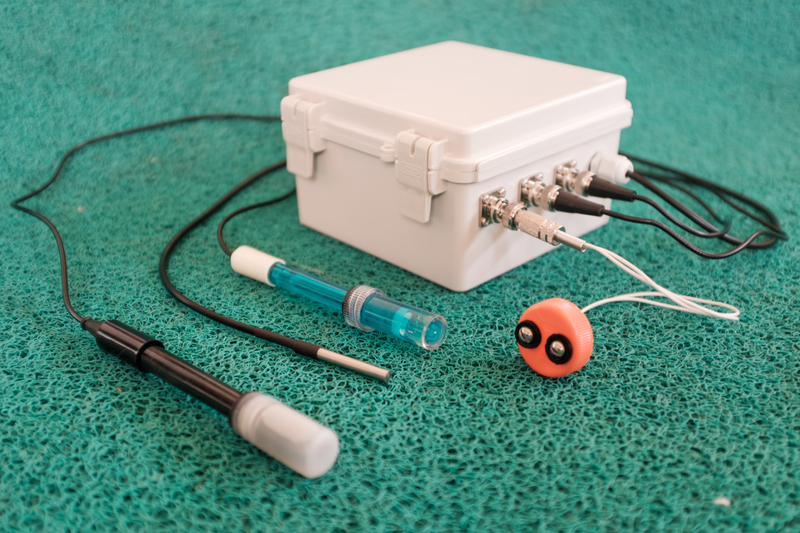
\includegraphics[width=300pt]{img/mae-dagua.jpg}
			\end{center}
			\caption{Mae d'Agua (source : Public Lab)}
		\end{figure}
		Parmi les différentes sources de données du projet, on peut notamment citer Mae d'Agua, un matériel ouvert qui permet de surveiller la qualité de l'eau. Un réseau de capteurs sans fils (WSN) qui récupère les informations relatives à la qualité de l'eau telles que la conductivité électrique, le pH, le potentiel d'oxyréduction (OPR), la température, la pression barométrique ainsi que la température du capteur. Cet équipement peut être utilisé pour surveiller la qualité de l'eau dans des boîtes à eau, des citernes et réservoirs ainsi que les corps d'eau à faible débit. Inspiré du capteur "Riffle", ce matériel a été développé en collaboration avec Public Lab (réseau américain de science citoyenne) ainsi que Dev Technologia, une startup de Sao Paulo University. Les données recueillies sont envoyées à un serveur via le réseau de téléphonie mobile. Les relevés sont effectués à une fréquence d'un par heure. Il est nécessaire de nettoyer régulièrement les capteurs afin d'éviter que les relevés ne soient erronés à cause de l'accumulation de débris. Il s'agit d'un projet open source et open hardware, les fichiers et firmware sont disponible sous licence MIT. \\
		L'équipement est modulaire et comporte 3 modules :\\
		\begin{enumerate}
			\item Le premier module est un Arduino Mega. Il gère le traitement des données ainsi que l'alimentation en énergie depuis une source externe.
			\item Le deuxième module est une coque Arduino conçue grâce à la plateforme Eagle. Cette coque dispose d'un capteur de pression barométrique et de connecteurs permettant d'ajouter les capteurs de pH, température, OPR et de conductivité. Cette conception modulaire permet d'optimiser le rapport coût-bénéfices en fonction de l'application projetée.
			\item Le troisième module permet la communication au travers du réseau téléphonique mobile pour envoyer les données au serveur.
		\end{enumerate}
		Le projet est soutenu par Google et par des institutions et entreprises locales.

	\subsection{Reef Citizen Science Alliance}
		Ce projet regroupe des citoyens qui aident à collecter des données sur la grande barrière de corail, en Australie. Les volontaires peuvent participer à des ateliers de formation qui s'adressent aux personnes ayant des connaissances faibles ou modérées sur les coraux (voir \textit{reefcitizenscience.org}). Ils apprennent comment effectuer les relevés de façon simple. Il existe de nombreuses façon de contribuer sans effectuer cette formation, par exemple en signalant des espèces marines particulières lors d'une session de plongée ou de snorking au moyen d'une application pour smartphone. L'application permet également de signaler des évènements en temps réel et de voir ce que les volontaires peuvent faire autour d'eux pour contribuer. \\
		Les résultats de ces relevés sont largement utilisés par la Great Barrier Reef Foundation qui contribue à financer de nombreux projets de préservation et de  restauration de la barrière de corail Australienne.
	
	\subsection{World Water Monitoring Challenge}
		Le WWMC est un projet de EarthEcho International (voir \textit{earthecho.org}). Cet évènement, conduit chaque année entre mars et décembre, réunit plus de 1'500'00 participants dans un total de 146 pays. L'idée est d'équiper et former les citoyens afin qu'ils surveillent leurs points d'eau locaux tout autour du monde avec pour le moment 77'685 endroits surveillés. La sensibilisation et l'incitation à la surveillance pour protéger les ressources hydriques sont les points clés de ce projet. \\
		Les citoyens participent par plusieurs voies :
		\begin{itemize}
			\item Par la surveillance des points d'eau à l'aide de kits.
			\item Par le partage des données au travers d'une plateforme et des réseaux sociaux.
			\item Par l'utilisation des informations pour protéger les ressources hydriques vulnérables. 
		\end{itemize}
		Les kits comprennent : 1 livre d'instruction, 1 récipient pour les échantillons, 1 tube de à essais de pH, 1 fiole de d'oxygène dissous, 2 bandes de température, 50 comprimés de réactif au pH, 100 comprimés de réactif d'oxygène dissous, 1 disque de Secchi et 1 nuancier pour l'interprétation des résultats (DO, pH, turbidité). Les kits sont conçus pour permettre d'effectuer 50 tests et coûtent environ 50 dollars. Le projet permet également à certaines organisations, sous conditions, d'obtenir gratuitement des kits.
	
	\subsection{FreshWater Watch}
		Le FreshWater Watch (voir \textit{freshwaterwatch.thewaterhub.org}) ambitionne de monitorer un maximum de petits corps d'eau tout autour du monde. Ceux-ci sont rarement déjà sous surveillance et sont souvent déjà affectés par différents facteurs. Ce projet propose d'établir une carte mondiale en partenariat avec toute organisation, association ou communauté prête à partager et échanger des informations. Ils travaillent par exemple en collaboration avec le Riverfly Partnership à l'origine de la Riverfly Monitoring Initiative. Ce projet se montre ouvert à tout type de contribution, et particulièrement les observations visuelles (végétation, activités humaines, niveau d'eau, utilisation des terres autour, vie animale, vitesse d'écoulement et couleur de l'eau, présence d'algues, sources visibles de pollution) au moyen de photographies. Comme les informations visuelles ne permettent pas à elles seules de déterminer la qualité de l'eau, il est important de les compléter au moyen de tests chimiques et d'analyses de bio-indicateurs. FreshWater Watch se monstre particulièrement attentif à deux facteurs :
		\begin{enumerate}
			\item La présence excessive de nutriments dans l'eau, qu'ils considèrent comme le plus grand problème à large échelle. Les nutriments sont nécessaires à la vie marine mais peuvent créer des problèmes lorsqu'ils sont en surabondance. Par exemple, une quantité anormale de nutriments peut favoriser la croissance d'algues qui vont réduire la quantité d'oxygène disponible dans l'eau, ce qui peut mener à l'apparition de "Dead Zones".
			\item La turbidité de l'eau au moyen d'un tube de Secchi pour mesurer le nombre de particules dans l'eau. En croisant les données des nutriments et de la turbidité, on peut suggérer s'il y a eu une prolifération d'algues ou si le ruissellement transporte trop de pollution dans le plan d'eau. La turbidité est également liée à la quantité d'oxygène dans l'eau. Les particules dans l'eau ont un effet sur la vie aquatique puisqu'elles obstruent les branchies et affectent le développement des oeufs.
		\end{enumerate}
		\begin{figure}
			\begin{center}
				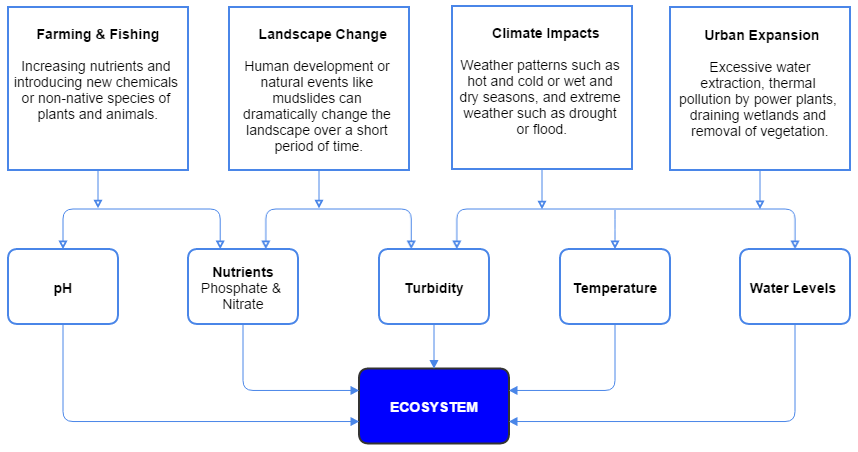
\includegraphics[width=300pt]{img/ecosystem-flowchart.png}
			\end{center}
			\caption{Schéma simplifié des mesures effectuées et des facteurs impactants un écosystème (source : FreshWater Watch)}
		\end{figure}
		Le projet permet d'obtenir un kit pour tester localement la qualité de l'eau. On peut ensutie mettre en ligne les résultats sur le site internet du projet.\\
		Les données mises en ligne par les volontaires sont disponibles gratuitement en ligne sous la forme d'une carte interractive.
		
	\subsection{NAWMS}
		On a constaté que donner des informations précises et en temps réel aux usagers sur leur consommation d'essence avait permit de les sensibiliser et de mieux conserver les réserves. Le Non-intrusive Autonomous Water Monitoring System \cite{kim_nawms:_2008} vise à appliquer cette philosophie à la consommation d'eau : en donnant aux gens la possibilité de savoir ce qu'ils consomment et comment, on leur donne les informations nécessaires pour adapter leurs habitudes à un mode plus économe et renouvelable. Nous n'avons en effet pas idée de ce qu'est une consommation considérée comme "faible", "modérée" ou "forte" en tant que particulier.\\
		Le NAWMS est un système de surveillance de la consommation de l'eau qui est non intrusif et autonome pour sa calibration. Il se base sur la propagation des vibrations le long des tuyaux qui est proportionnelle au débit d'eau.\\
		Ce système est basé sur une archiecture deux-tiers :
		\begin{figure}
			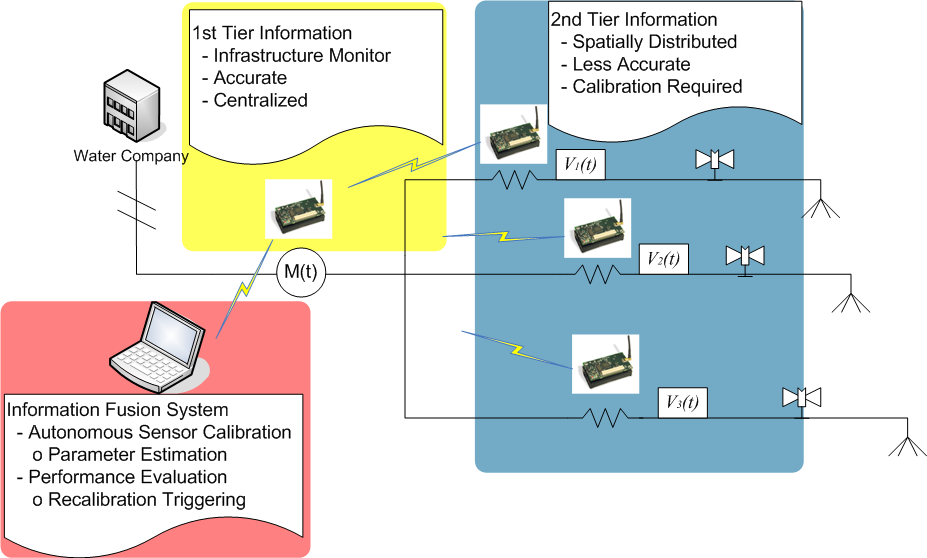
\includegraphics[width=200pt]{img/nawms.png}
			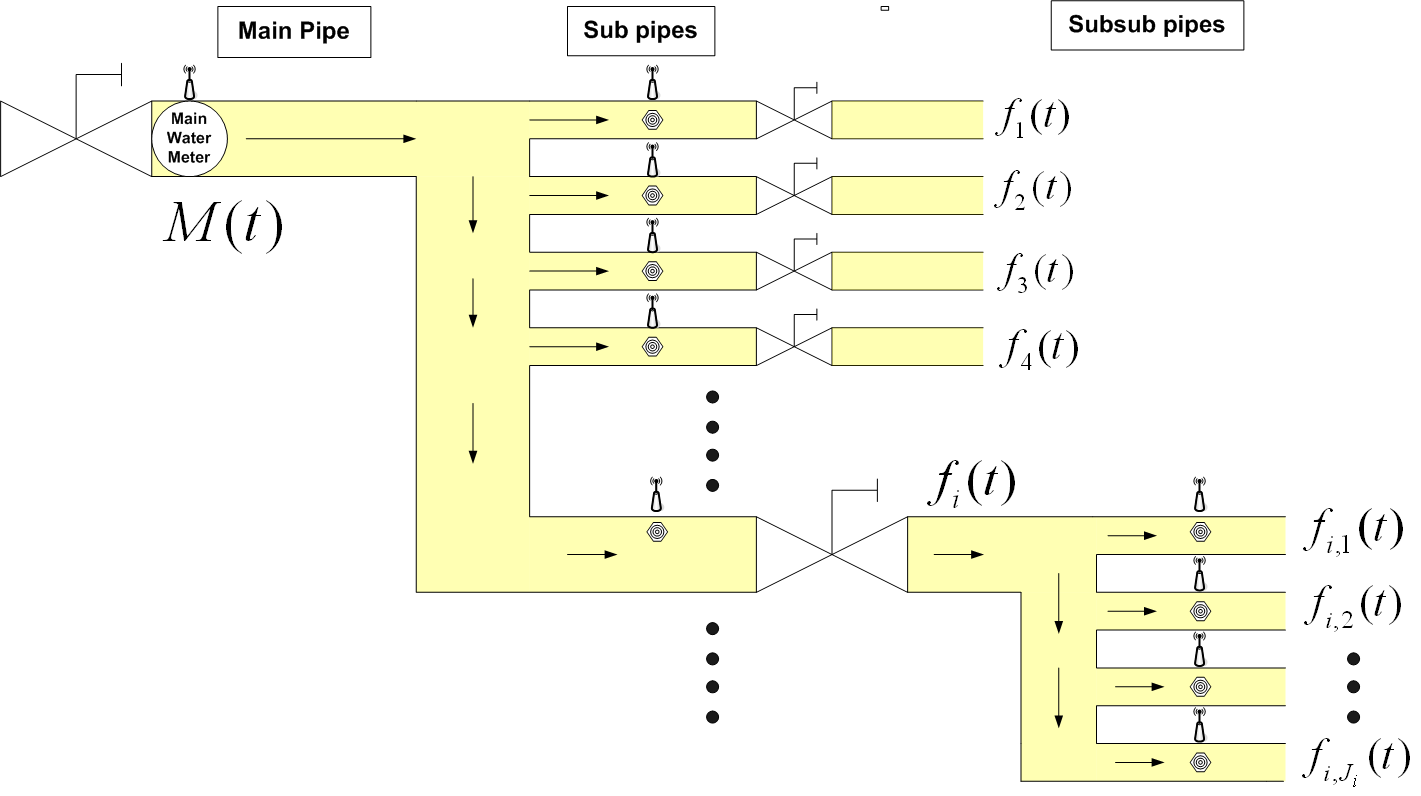
\includegraphics[width=200pt]{img/nawms2.png}
			\caption{Architecture du système NAWMS (source : \cite{kim_nawms:_2008})}
		\end{figure}
		\begin{enumerate}
			\item Le premier tier est le fournisseur du service. Celui ci est précis mais centralisé et ne dispose donc pas d'une répartition spatiale fine. Il s'agit également d'une source fiable dont l'utilisateur n'a pas à se préoccuper de la maintenance, de la précision ou du bon fonctionnement. De plus, il est considéré comme toujours disponible et permet au système de se calibrer continuellement.
			\item Le second tier est l'ensemble des capteurs de vibrations répartis sur les différents tuyaux. Ceux-ci sont moins précis mais sont disribués finement spatialement. Cette architecture en deux-tiers permet d'obtenir des résultats globaux et locaux précis.
		\end{enumerate}
		Le système est capable de modéliser le bruit externe, les limitations et caractéristiques physiques ainsi que les performances. La métrique de performance est utilisée pour calibrer l'ensemble du système automatiquement sans avoir recours à une intervention manuelle pour la maintenance. Ce calibrage est rendu possible par la reformulation des équations d'optimisation sous une forme résolvable en un temps polynomial. Les différents paramètres de ces équations sont : la vibration mesurée, la constante de propagation des vibrations du tuyau $j$ au tuyau $i$ (propre au matériaux utilisés) et la vibration induite par le débit d'eau sur le tuyau $j$.
		\begin{figure}
			\begin{center}
				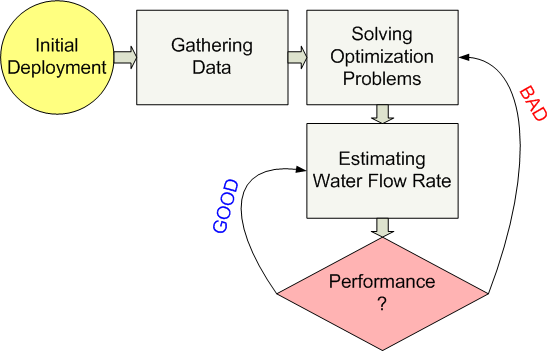
\includegraphics[width=200pt]{img/nawms3.png}
			\end{center}
			\caption{Calibrage continu du NAWMS (source : \cite{kim_nawms:_2008})}
		\end{figure}
		Les résultats des tests effectués sur plusieurs tubes de matières et diamètres différents sont précis et démontrent l'intérêt de cette approche.\\
		Les capteurs à vibrations peuvent être installés sur n'importe quel tuyau visible sans avoir à faire appel à un plombier ou à effectuer de lourds travau de rénovation. Il devient donc possible pour n'importe qui de connaître avec précision les dépenses en eau de chaque source (douche, robinet, lave linge, ...) pour adapter sa consommation et/ou détecter d'éventuelles fuites. 
	
	\subsection{Riverfly Monitoring Initiative}
		Ce projet (voir \textit{riverfly.org}), réalisé aux Royaumes-Unis, réunis de nombreux acteurs tels que pêcheurs, authorités compétentes comme le ministère de l'environnement, scientifiques et entomologistes dans le but de protéger la qualité de l'eau des rivières, de mieux comprendre les populations des mouches de rivière et de conserver leur habitats. Ces insectes jouent un rôle fondamental dans les rivières, en particulier concernant l'alimentation de certains poissons et chauves-souris car ils font partie du plancton aérien. Ces insectes, apparus au Carbonifère (il y a environ 300 millions d'années) sont extrêmement sensibles à la pollution lumineuse et chimique, notamment par les pesticides. On compte parmi ces espèces les éphémères, les plécoptères et les trichoptères. Ils passent la plus grande partie de leur vie au stade larvaire, dans l'eau. De ce fait, les facteurs tels que le débit d'eau, sa qualité ou encore son niveau ont un impact majeur sur ces espèces. Leurs caractéristiques les rendent particulièrement pertinentes en tant qu'indicateurs lors d'études de la qualité de l'eau. Par exemple, lors du rejet d'eaux usées, un des bio-indicateurs de pollution peut être les populations de certaines espèces de plécoptères puisque celles-ci, sensibles à la quantité d'oxygène dissous, vont chuter brusquement. \\
		Le Riverfly Partnership organise des journées de formation pour les clubs de pêche et autres groupes de personnes concernées par la surveillance des cours d'eau. Les pêcheurs disposent d'une position privilégiée pour surveiller la qualité et l'état des cours d'eau dans lesquels ils pêchent. Ils sont nombreux a exprimer un intérêt à pouvoir eux-même effectuer les vérifications de l'eau. Les conditions pour participer à la RMI est d'avoir une personne prête à devenir coordinatrice locale ainsi que des membres prêts à suivre la journée des ateliers de formation qui consistent en diverses présentation et démonstrations pratiques de l'utilisation du matériel. 
		Ce projet préconise une fréquence de relevés mensuelle, ce qui rend les mesures sensibles aux fluctuations saisonnières et aux cycles naturels. On estime à une heure le temps nécessaire par volontaire pour effectuer les prélèvements. Les kits de prélèvement contiennent : un filet de 25cm (maille de 1mm), un grand plateau, un seau, un bac diviseur en 8 parties, une pipette, une loupe, une petite cuillère, un pinceau et le guide pratique de l'utilisation du matériel.\\
		Les résultats sont disponibles librement sur leur site web et permettent de visualiser au moyen d'une carte les endroits ou sont effectués les relevés. Ces données sont également partagées aux différents organismes gouvernementaux en charge de la protection et de la restauration de  l'environnement.
	
	\subsection{Restoration Assessment Initiative}
		La multitude de projets de monitoring de la qualité de l'eau a permit de démocratiser la participation citoyenne aux projets de surveillance locaux, notamment sur la détection de la pollution sur de larges périodes de temps. Bien que les différents acteurs des initiatives partagent un but commun, à savoir améliorer la qualité de l'eau, les conditions de pêche à la ligne et la biodiversité, il n'existe à ce jour aucun projet citoyen visant à évaluer le succès de la restauration qui vise à atteindre les buts énoncés ci-dessus \cite{huddart_citizen_2016}. La Restoration Assessment Initiative propose un modèle standardisé pour évaluer la réponse biotique aux projets de restauration de l'environnement. Le but est de permettre la mise en place d'une base de donnée à large échelle permettant de connaître, à terme, les plus gros facteurs de succès et d'échecs des projets de restauration. Nos socitétés sont fortement influencées par les services que nous fournit l'écosystème, c'est pourquoi il est important de rétablir l'intégrité des cours d'eau et de stoper le déclin des espèces. Cela pose cependant un nombre non négligeable de challenges.
		Dans les zones dégradées, l'un des principaux problème est le manque de diversité des habitats. Cette donnée est critique puisqu'elle va contraindre la capacité d'un écosystème à se rétablir. En augmentant l'hétérogénéité des habitats, on aide à restaurer la biodiversité et l'intégrité de l'écosystème. Cette théorie n'a cependant pas beaucoup de preuves : les améliorations locales sont souvent surpassées par les études à large échelle et, à cause du manque de ressources, de temps et d'argent, 90\% des projets de restauration ne sont pas surveillés (USA, Australie, Europe) autrement que par une évaluation visuelle. Ces causes pourraient être mitigées par l'utilisation de sciences citoyennes en utilisant des protocoles standardisés de surveillance et des méthodes de mesures quantitatives pour mesurer les critères appropriés. Déployé à large échelle, cette approche offrirait une toute nouvelle perspective avec un coût relativement faible grâce aux avantages précités des sciences citoyennes.\\
		\begin{figure}
			\begin{center}
				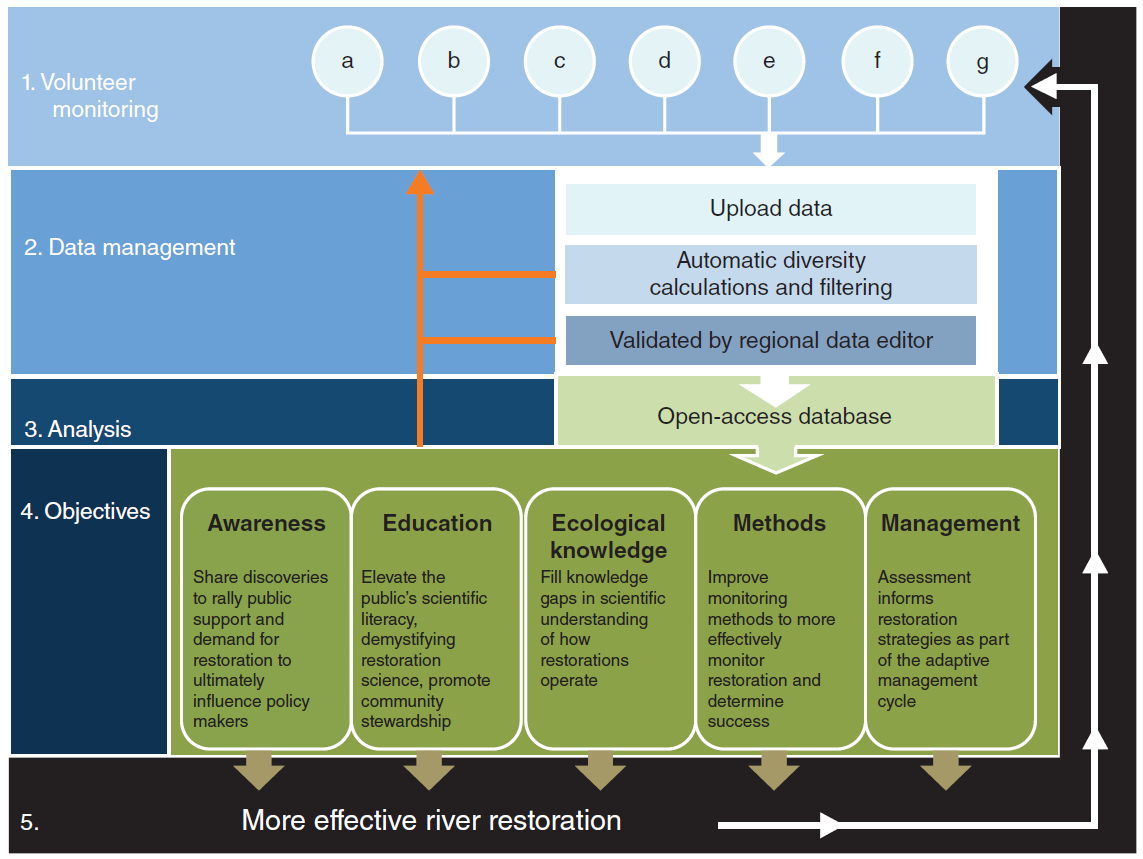
\includegraphics[width=300pt]{img/RAI.png}
			\end{center}
			\caption{RAI framework (source : \cite{huddart_citizen_2016})}
		\end{figure}
		Les projets de restauration seraient ainsi plus personnalisés et les différents résultats, qu'ils soient positifs ou négatifs, seraient utilisés dans un but de guider les efforts et la recherche.
		Le RAI prend la Riverfly Monitoring Initiative en modèle mais ajoute l'analyse statistique Before-After Control-Impact (BACI) pour contrôler un point à la fois dans le temps et l'espace. L'anlyse BACI rend les données robustes puisqu'elle permet de distinguer les effets de la restauration et ceux des fluctuations saisonnières. L'étude doit cependant être menée sur plusieurs années puisque les prélèvements ne se font plus mensuellement mais annuellement. Les mesures effectuées sont plus nombreuses et le nombre de taxons évalués est plus grand. La différence fondamentale entre le modèle proposé et l'approche de la RMI est que les données sont aggrégées pour comprendre les causes de succès ou d'échecs des projets de restauration. Ceci permet d'investir les ressources pour influencer positivement les futurs projets et de compléter la base de données au fur et à mesure de l'évolution des projets.
		
	\subsection{Clean Air Carolina}
		Le Clean Air Carolina (voir \textit{cleanaircarolina.org}) est une initiative qui vise à améliorer la qualité de l'air en Caroline du nord. Pour atteindre ce but, ils soutiennent entre autre un projet de sciences citoyenne dans lequel les volontaires récoltent des données à la fois à certains endroits fixes mais aussi en mouvement, par exemple à vélo ou en transports publics. Cette approche est motivée par le fait que la qualité de l'air peut changer drastiquement d'un côté à l'autre d'une ville, et une exposition prolongée aux particules peut provoquer des problèmes de santé. Les citoyens peuvent participer aux campagnes de sensibilisation, aux évènements de surveillance pour récolter des données ou héberger un capteur pour surveiller la qualité de l'air. Ceux-ci coûtent 450 dollars américains et peuvent être payé par d'autres citoyens, par l'hôte ou par un sponsor. Les résultats sont disponibles librement sur le site web du projet au moyen d'une carte interactive.
		
	\subsection{Air Pollution Map}
		Aux Pays-Bas, des citoyens ont pu aider à cartographier la pollution en utilisant leur smartphone. Les volontaires mesuraient les quantités d'aérosols en suspension dans l'air. La plupart de ces particules sont surveillées et régulées par l'Union-Européenne dans le cadre de la "Air Quality Directive". La plupart du temps, les études sont menées par un groupe d'experts ou par satellites. Cette approche présente le défaut d'être peu distribuée spatialement et avec une faible résolution (10km) pour les images satellite. Il est donc difficile d'établir une carte à la fois globale et précise. Dans le cadre du projet, les volontaires ont attaché un petit périphérique à leur smartphone qui permet d'effectuer les mesures et profite également de certains capteurs du smartphone tel que le GPS. La communication est assurée au moyen d'une application.\\
		Les observations sont faîtes avec le périphérique installé au travers de l'appareil photo du smartphone, ce qui réduit la qualité des données par rapport à une station professionnelle. Cependant cet aspect est compensé par la large quantité d'échantillons récoltés. L'étude, menée en 2013, a permis de récolter près de 10'000 observations qui ont servi à créer une carte pour montrer les variations au niveau national. Ces observations ont également permis d'étudier l'évolution des concentrations heure par heure dans les grandes villes avec une résolution cinq fois meilleure qu'une étude menée par satellite. Les résultats de l'étude menée par les citoyens volontaires ont étés comparés à ce qui avait été mesuré par l'une des stations professionnelles, et ils étaient de très bonne qualité. Cela suggère qu'une surveillance de la qualité de l'air par smartphone par une communauté bien coordonnée est potentiellement plus efficace que si elle était basée sur la surveillance par des stations fixes ou par satellites.
		
	\subsection{Autres projets, logiciels et applications}
		Les citoyens volontaire peuvent également contribuer à des projets de sciences citoyennes par le biais d'applications comme Epicollect, INaturalist, Water Reporter, Project Noah, NatureBytes etc.\\
		INaturalist propose une approche ou chacun peut photographier ses observations personnelles et les envoyer à la communauté par exemple au moyen de son smartphone mais l'application fonctionne sur tous les appareils. La communauté se charge alors d'identifier et répertorier le specimen. Toutes les données sont partagées avec le l'Établissement pour l'Information sur la Biodiversité Globale (Global Biodiversity Information Facility - GBIF) qui répertorie chaque information reçue avec un total actuel d'un peu plus d'un milliard d'enregistrements.\\
		Epicollect permet à tout un chacun de créer sa propre application de collection de données et de la partager simplement sur tous les appareils qui peuvent l'installer ou disposent d'un accès internet. Les applications créées ne nécessitent pas de connexion active à internet pour fonctionner, seule la transmission finale demande à établir une connexion au serveur. Les données peuvent ensuite être contrôlées, filtrées, modifiées et visualisées. \\
		Water Reporter est une application pour smartphone qui met à disposition des fonctions pour capturer et partager des observations visuelles géolocalisées des points d'eau et de leur état à large échelle. La communauté est surtout présente aux États-Unis.\\
		Project Noah permet également de répertorier ses observations et de les partager, mais celles-ci ne sont pas exclusivement dédiées aux points d'eau ou aux espèces marines. Il n'existe par contre pas d'application pour Project Noah, chaque photo doit être uploadé sur le site manuellement.\\
		NatureBytes est un boitier  étanche qui permet de photographier les éléments qui passent devant. Cet équipement a été pensé pour capturer des images d'animaux, et particulièrement pour ceux difficiles à observer à cause de leur caractère craintif ou discret. Le boitié en plastique intègre tout le matériel et logiciel nécessaire pour garantir au Raspberry Pi embarqué de pouvoir prendre les photos de façon autonome durant plusieurs jours. Le Raspberry Pi permet de modifier les périphériques utilisés mais le boitier est de conception fixe.

\section{Conclusion}\label{sec:conclusion}

% use section* for acknowledgement
\section*{Remerciements}
	A Monsieur François Grey et Madame Rosy Mondardini pour les idées, leur relecture et leur aide en général lors de la rédaction de ce document.

\bibliographystyle{alpha}
\bibliography{soa} %%% soa.bib is the file containing bibliographic entries
\fancyhf{}


% that's all folks
\end{document}


